\section{Example SmartHome Scenarios}
To understand how our device could be used to interact with smart appliances, we also asked all study participants to work through a concrete scenario. The main goal was to obtain qualitative feedback on the usability and utility of our device with more realistic tasks.

\begin{figure}[t]
\centering
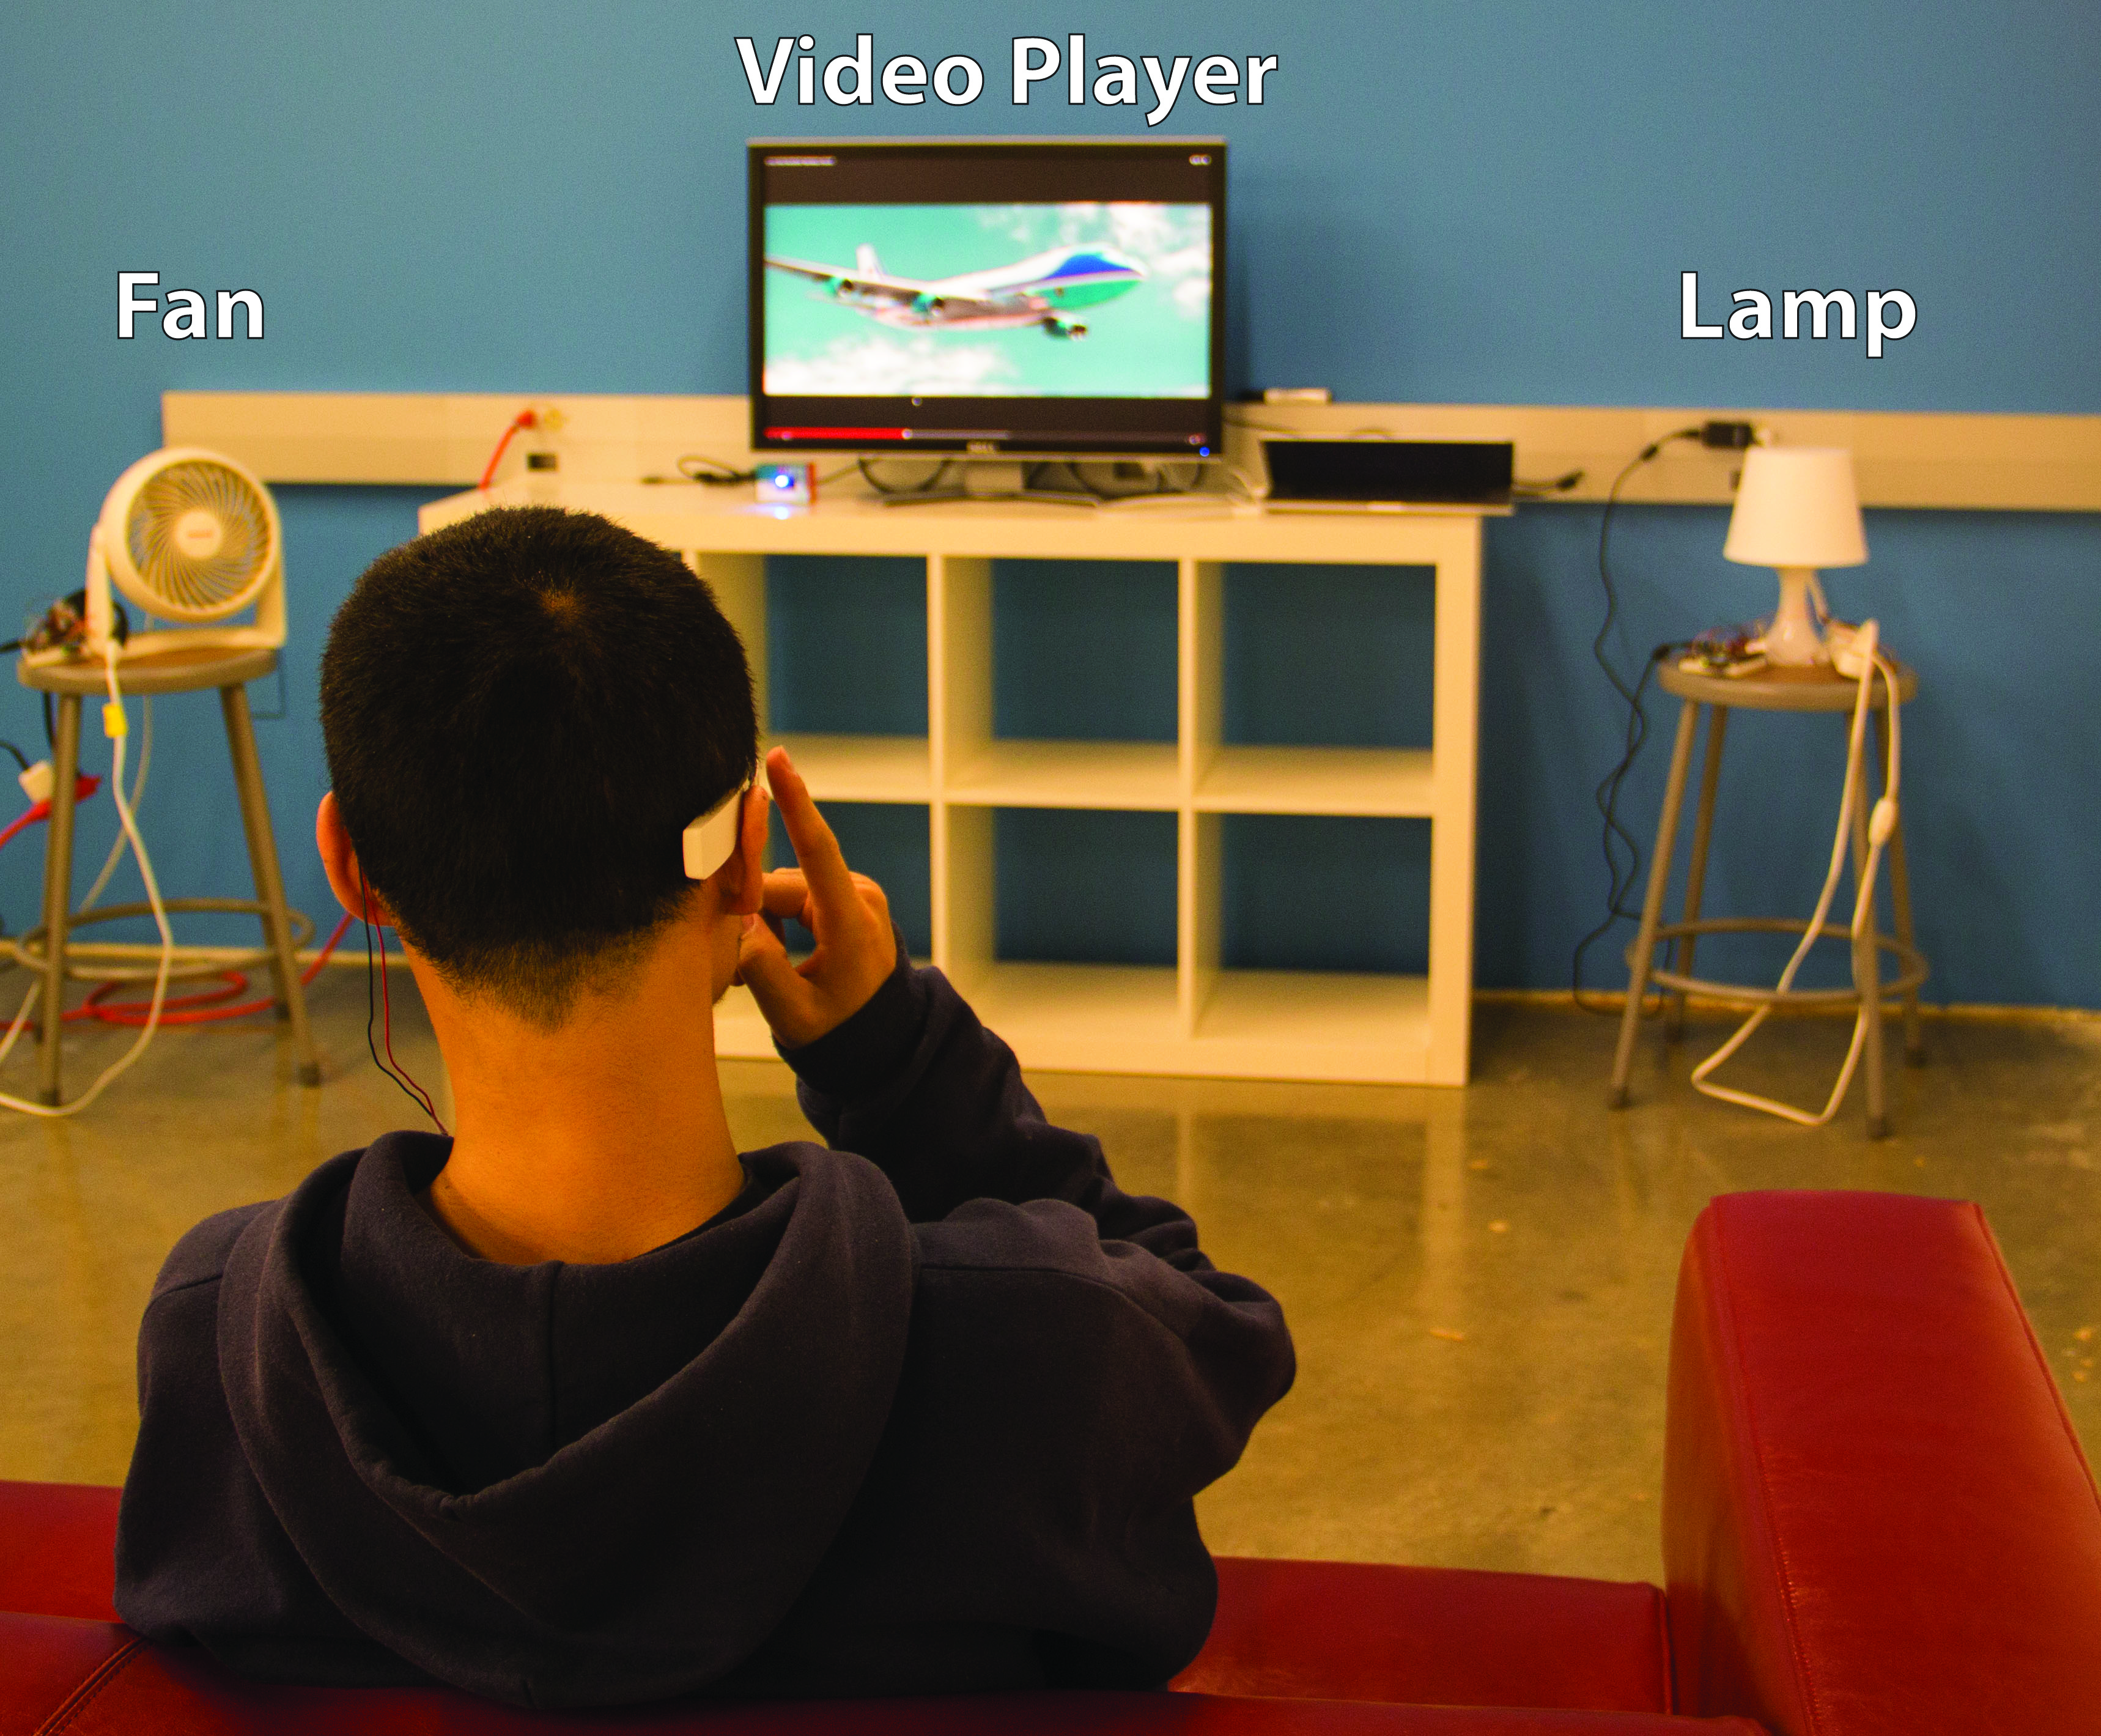
\includegraphics[width=1.0\columnwidth]{figures/smarthome-scenario.jpg}
\caption{In the targeting study, participants had to find and select one of 10 targets in a lab environment.}
\label{fig:smarthome}
\end{figure}

\subsection{Methodology}
We recreated a living room environment that had three (four?) controllable appliances: a fan, a lamp, and two laptops functioning as an audio and video player, respectively (see Figure~\ref{fig:smarthome}). The fan and lamp had binary controls: they could be switched on or off. The laptop had multiple parameterized functions: participants could start, pause, stop, and rewind  video and audio, and adjust volume.

We then asked users to work through the following script:

\small{
\begin{enumerate}
\item Turn off the lights as you want to watch the movie in a darkened room.
\item You feel a little hot in the room, so you turn on the fan
\item You connect to the Smart TV and start playing the movie. 
\item The volume seems too soft to hear over the fan- turn it up a bit. 
\item After a while, you want to take a break to get a snack. Pause the movie. 
\item When you come back, you've forgotten what was said last - rewind by ~30 seconds and restart the movie. 
\item You stop the movie and turn the lights back on.
\item You want to listen to some music.
\item After awhile, you stop the music
you turn off the fan and leave the room.
\end{enumerate}}

\subsection{Qualitative results}

\bjoern{Here we should either describe a couple of example scenarios we've built, or get some students to run through realistic control tasks based on those scenarios - e.g.: ``Dim the light to 20\% and then start the movie, turn up the volume to 80\%."}
